\chapter{Results}\label{chap:results}
The metrics described in Chapter\ref{chap:design} have been collected for the created CC UI library. Using these metrics, we are able to compare the CC UI library to the original Angular components, the various JS framework wrappers, and various other UI libraries. In the following sections, the various metrics are broken down, and the results are compared between the various libraries.

\section{Render Time}
The render time metric allows us to evaluate the direct performance impact on users once the page has loaded. We first compare the CC UI library to the original Angular components and the other JS framework wrappers. This allows us to evaluate the performance impact added by the process of conversion to Web Components, as well as the performance impact added by the JS framework wrappers. After this, we compare the CC UI library to the UI libraries listed in Table~\ref{tab:design:ui-libraries}, allowing us to evaluate the performance of the CC UI library relative to UI libraries as a whole.

\subsection{Cow Components}
As mentioned in Chapter~\ref{chap:experimental-setup}, we have measured three basic components in particular that every UI library contains. These are the Button, Switch, and Input. We have measured the time needed to render 1 instance, 10 instances, and 100 instances of this component. The various render times for the cow-components UI libraries with these numbers of components can be seen in figures~\ref{fig:results:render-time-cow-1},~\ref{fig:results:render-time-cow-10}, and~\ref{fig:results:render-time-cow-100} respectively. We first take a look at the single-component render times. When we compare the performance of the CC UI library with the original Angular components, we find the CC UI library's median render time to be 81\% and 100\% higher for the Input and Switch components, respectively, with the mean render time for the Button being 41\% lower. Other than the Angular wrapper's Button (which is 100\% slower), the wrappers' render times are very similar. The React and Svelte Button rendering times are 6\% and 12\% lower, respectively, with both the Input and Switch render times being between 172\% and 190\% higher. From this, we can conclude that, although there is a full Angular root running for each component, the performance impact for a single component is minimal. Now taking a look at the render times for 10 and 100 components, we start to see some big differences. The Web Components version can still keep up with the original components when it comes to rendering 10 components, being 5\% faster, 144\% slower, and 111\% slower for the Button, Input, and Switch components, respectively. When rendering 100 components instances, however, it is eclipsed by the original components. Render times are 250\%, 393\%, and 265\% slower for the Button, Input, and Switch, respectively. It seems that the impact of creating a new Angular root for each component does become significant with many components.
Additionally, the render times for the various JS frameworks start to differ quite a lot. We see a trend of the React and Svelte wrapper growing further away from the Web Components version, with the average of the component render times increasing by 339\% for the React wrapper and 597\% for the Svelte wrapper. The Angular wrapper moves away even further, with the average of its component render times increasing by 735\%. It seems that the performance impact for rendering a relatively small amount of components is minimal, while it scales up relatively quickly with a greater number of components. The fact that picking a JS framework to develop in is especially interesting, potentially costing a difference of 150ms over Web Components or 50ms over a different framework.

\begin{figure}[h]
  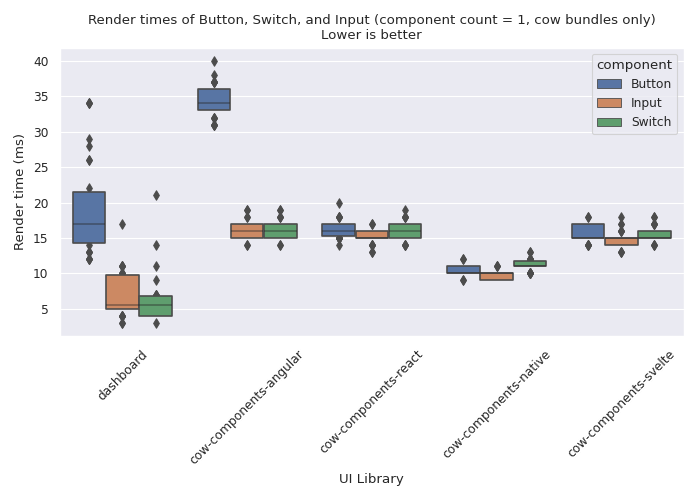
\includegraphics[width=\columnwidth]{plots/render-time-cow-1.png}
  \caption{Render times of a single Button, Switch, or Input component (CC UI only)}
  \label{fig:results:render-time-cow-1}
  \centering
\end{figure}

\begin{figure}[h]
  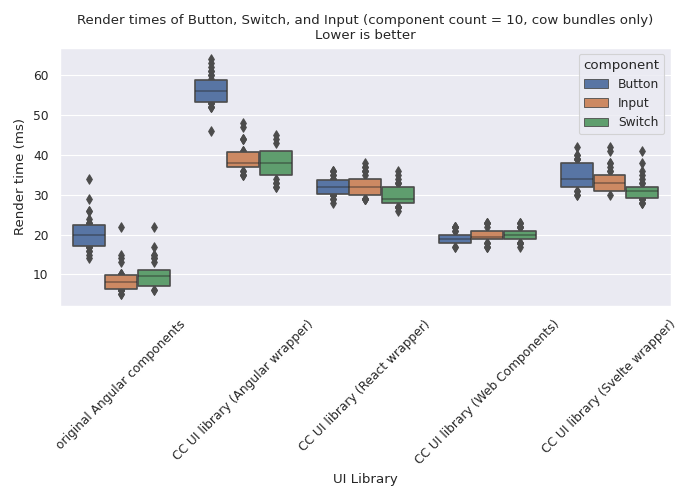
\includegraphics[width=\columnwidth]{plots/render-time-cow-10.png}
  \caption{Render times of ten Button, Switch, or Input components (CC UI only)}
  \label{fig:results:render-time-cow-10}
  \centering
\end{figure}

\begin{figure}[h]
  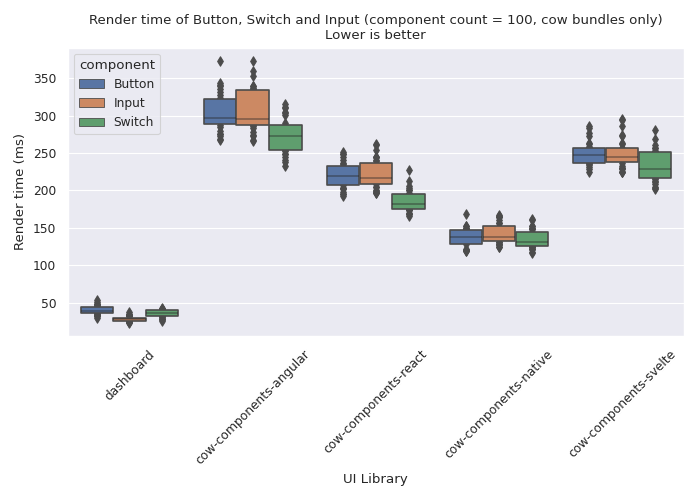
\includegraphics[width=\columnwidth]{plots/render-time-cow-100.png}
  \caption{Render times of one hundred Button, Switch, or Input components (CC UI only)}
  \label{fig:results:render-time-cow-100}
  \centering
\end{figure}

\subsection{UI Libraries}
We now compare the render times of the various UI libraries. Since the number of UI libraries we are comparing is very high (coming in at 29 total), showing them all in one figure makes for a very cluttered view. Instead, we compare a single component at a time. We have chosen to discuss the Button component in this section, however a complete overview can be found in Figures~\ref{fig:appendix:render-time-cow-1},~\ref{fig:appendix:render-time-cow-10}, and~\ref{fig:appendix:render-time-cow-100}. The render times of the Button component for the various UI libraries for 1, 10 and 100 components can be found in figures~\ref{fig:results:render-time-all-1},~\ref{fig:results:render-time-all-10}, and~\ref{fig:results:render-time-all-100} respectively.

\begin{figure}[h]
  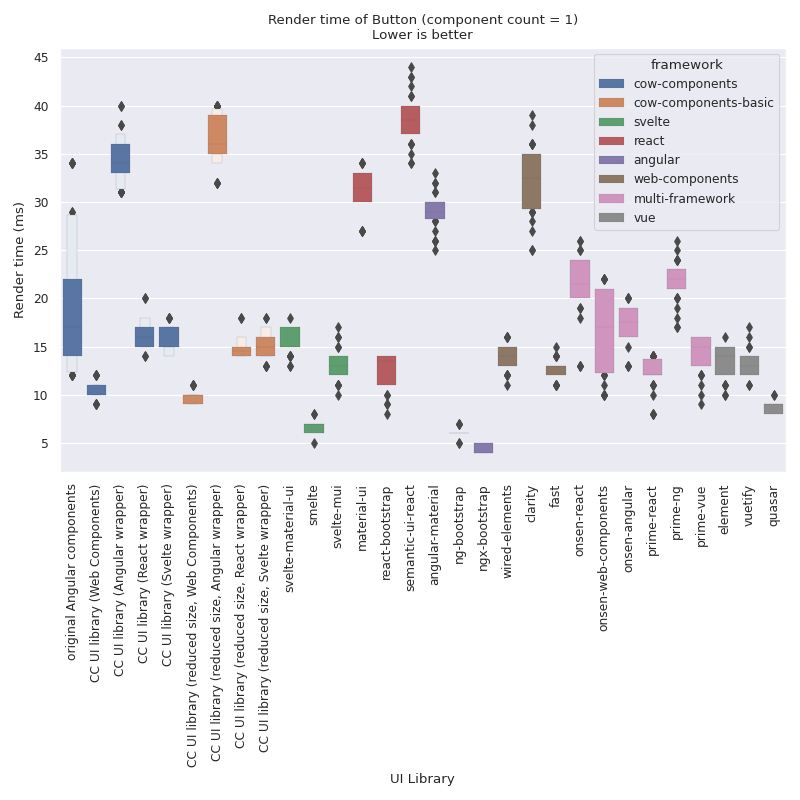
\includegraphics[width=\columnwidth]{plots/render-time-all-1-Button.png}
  \caption{Render times of a single Button. The reduced size CC UI library is the build of the library with less components, as described in Section~\ref{sec:experimental-setup:size}.}
  \label{fig:results:render-time-all-1}
  \centering
\end{figure}

\begin{figure}[h]
  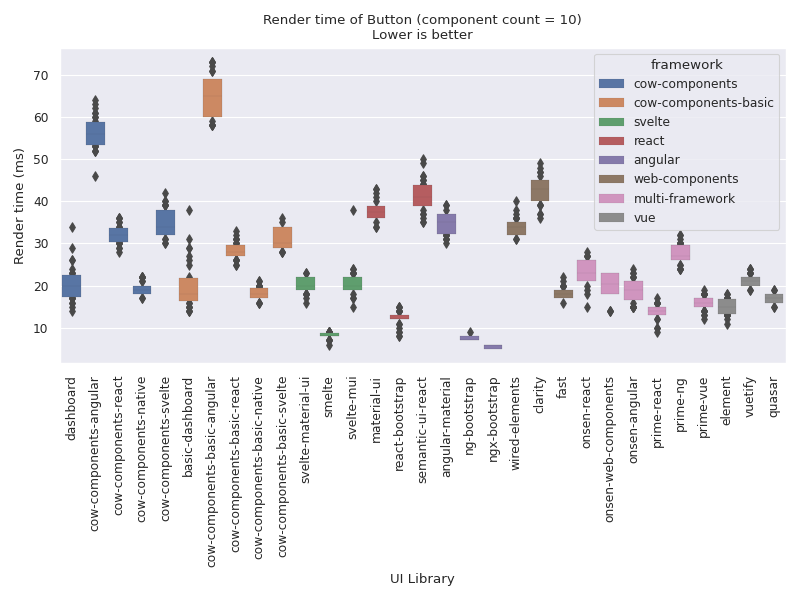
\includegraphics[width=\columnwidth]{plots/render-time-all-10-Button.png}
  \caption{Render times of 10 Buttons. The reduced size CC UI library is the build of the library with less components, as described in Section~\ref{sec:experimental-setup:size}.}
  \label{fig:results:render-time-all-10}
  \centering
\end{figure}

\begin{figure}[h]
  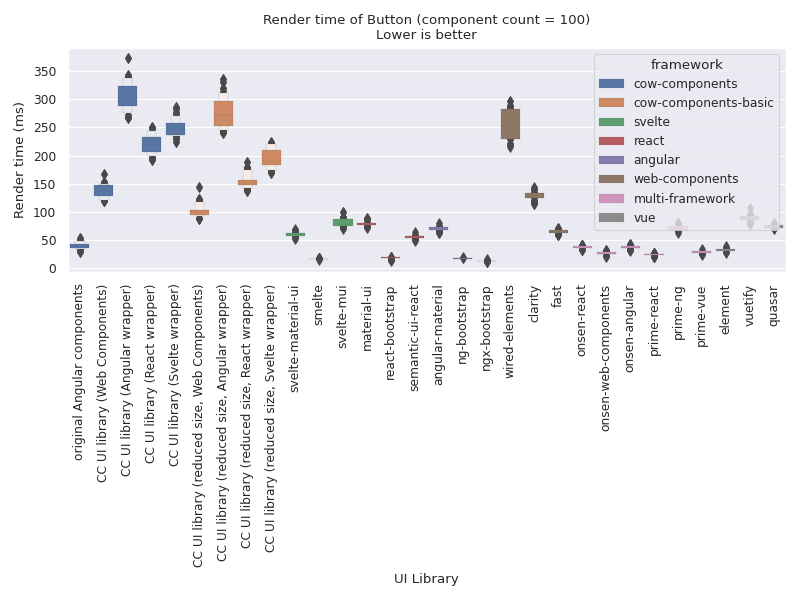
\includegraphics[width=\columnwidth]{plots/render-time-all-100-Button.png}
  \caption{Render times of 100 Buttons. The reduced size CC UI library is the build of the library with less components, as described in Section~\ref{sec:experimental-setup:size}.}
  \label{fig:results:render-time-all-100}
  \centering
\end{figure}

We, first of all, find that there are large differences in render times even within UI libraries that share the same framework. For example the render time for a button in \ver{react-bootstrap} is 57\% faster than \ver{material-ui} 64\% faster than \ver{semantic-ui-react}. In cases where this performance difference is relatively small, this has to do with the libraries themselves, but in a few cases, this has to do with the type of library. These libraries (\ver{react-bootstrap}, \ver{ng-bootstrap}, and \ver{ngx-bootstrap}) make use of a CSS framework, as laid out in section~\ref{sec:bg:ui-libraries}. As such, they are significantly faster and are essentially in a different category from the CC UI library, which is JS-based.

When we ignore these outliers, we can draw some conclusions on the average render times of the various frameworks. We first take a look at the single-component render times in Figure~\ref{fig:results:render-time-all-1}. We can see that Svelte UI libraries are generally swift, together having an average render time of 11.6ms. This falls in line with other performance benchmarks~\footurl{https://rawgit.com/krausest/js-framework-benchmark/master/webdriver-ts-results/table.html}. After this, Vue (12ms) and the UI libraries using Web Components (19,8ms) are the fastest. Interestingly, Web Components are slower than UI libraries using Svelte. Since Web Components are a native technology, one would be lead to believe that they would be faster. This might have something to do with how the authors of the UI libraries created their Web Components. It could be that their approach imposes a significant performance impact. The following frameworks when it comes to render time performance are Angular (29ms) and React (35ms). They are pretty close in performance, both being significantly slower than other frameworks. The previously mentioned performance benchmarks again support this.

We now apply our findings to the CC UI library JS framework wrappers. In our case, the Web Components version is the fastest simply because every other wrapper builds on top of this version. This means that it is impossible for another framework to be faster than it. We see this as well in the results, with the Web Components version coming in at 10ms. After that, the Svelte wrapper is the fastest, with a render time of 15ms. Interestingly, however, the React wrapper (16ms) is only slightly slower than the Svelte wrapper, while the Angular wrapper is significantly slower than both of them, coming in at 34ms. This is in contrast to what we just found, where both Angular and React were slow. It could be that the various internals of React that keep track of state and properties are slow. These are likely to be used a lot by regular React UI libraries, which need to handle their state entirely in React, while our React wrapper renders a component and passes it its properties once, making minimal use of methods exposed by React. In general, the CC UI library seems to be able to compete with the render times of other UI libraries, being faster than the vast majority of them.

\section{Load Time}
The load time metric allows us to evaluate the initial performance impact of the CC UI library. Again, we compare the various wrappers to each other as well as the original Angular components. As we elaborate on later, the Angular wrapper is significantly slower than any other UI library. For this reason, we split every figure into both a figure with and without the Angular wrapper. This should help show the scale of both this significant outlier while not reducing the scale's precision for other UI libraries.

\subsection{Cow Components}
The load time of the CC UI libraries can be seen in Figure~\ref{fig:results:load-time-cow-no-angular} (without the Angular wrapper) and Figure~\ref{fig:results:load-time-cow} (with the Angular wrapper). When we compare the load time of the CC UI library to the load time of the original 30MHz dashboard, we find that the CC UI library is significantly slower, coming in at 385ms compared to the 30MHz dashboard's 199ms. This is likely because the 30MHz dashboard has been optimized specifically for the initial load time. It loads the minimum amount of JavaScript needed to render the page. After this, other files are only loaded on an as-needed basis. The CC UI library, on the other hand, has to be contained in a single file. Splitting it up into multiple files and instructing third-party developers to have multiple JS bundles to make the CC UI library work would be a terrible developer experience. Concatenating the files into a single big bundle means all of the code has to be parsed and executed, slowing down execution by quite a lot.
Comparing the various wrappers to each other, we find the React and Svelte wrappers to have load times of 395ms and 434ms, respectively. This is only slightly slower than the CC UI library. The added load time is likely to be added by the JS frameworks themselves. Finally, we can see that the Angular wrapper is by far the slowest, with a load time of 4000ms. This is not entirely unexpected. As mentioned in Section~\ref{sec:case-study:ivy}, we had to disable AOT compilation for the Angular wrapper. This means all Angular compilation happens in the browser instead of during the compilation of the JS bundle. This is likely to be the reason why the Angular wrapper is so slow.

Taking a look at the reduced-size CC UI library, we find a loading time of 223ms for the CC UI library. This is only 12.6\% higher than the 30MHz dashboard. It appears that a significant portion of the loading was spent on these removed components. Further, the JS framework wrappers loading times are 588ms, 238m, and 277ms for the Angular, React, and Svelte wrappers, respectively. Again, the difference between the React and Svelte wrappers is minimal, with the Angular wrapper being significantly slower.

\begin{figure}[h]
  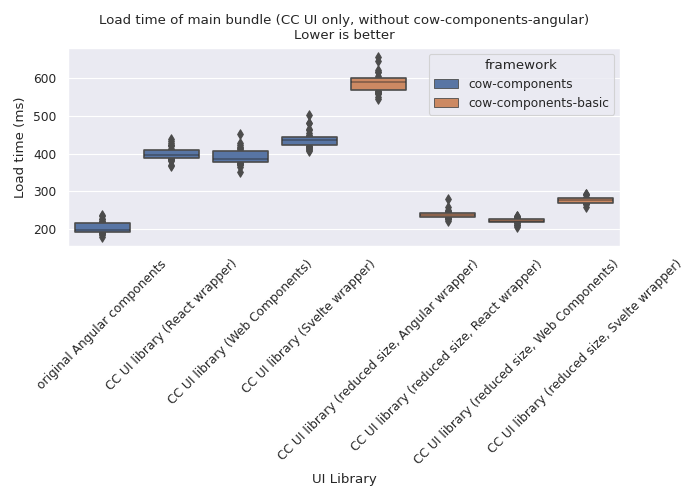
\includegraphics[width=\columnwidth]{plots/load-time-cow-no-angular.png}
  \caption{Load time of the main JS bundle (CC UI only, without Angular wrapper).}
  \label{fig:results:load-time-cow-no-angular}
  \centering
\end{figure}

\begin{figure}[h]
  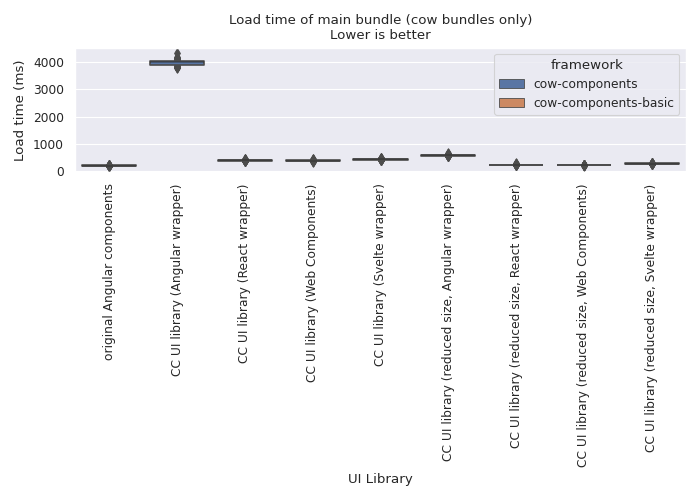
\includegraphics[width=\columnwidth]{plots/load-time-cow.png}
  \caption{Load time of the main JS bundle (CC UI only).}
  \label{fig:results:load-time-cow}
  \centering
\end{figure}

\subsection{UI Libraries}
The load times of other UI libraries can be seen in Figure~\ref{fig:results:load-time-all-no-angular} (without Angular wrapper) and Figure~\ref{fig:results:load-time-all} (with Angular wrapper). Other UI libraries largely differ in load time as well. Svelte UI libraries are by far the fastest, having an average load time of 2.64ms, followed closely by Web Components UI libraries at 11ms and React UI libraries with 22ms. After this, Vue UI libraries are the fastest, with a load time of 57ms. Finally, we have Angular, which with an average loading time of 106ms, is by far the slowest. Interestingly, we can see that the different distributions of multi-framework UI libraries follow this same pattern. For example the \ver{prime-ng} UI library is 329\% slower than the \ver{prime-react} UI library. Similarly, \ver{onsen-angular} is 167\% slower than \ver{onsen-react} and 308\% slower \ver{onsen-web-components}. This could also be one of the factors that are causing our Angular wrapper to be slower, although the lack of AOT compilation is still by far the most influential factor.

\begin{figure}[h]
  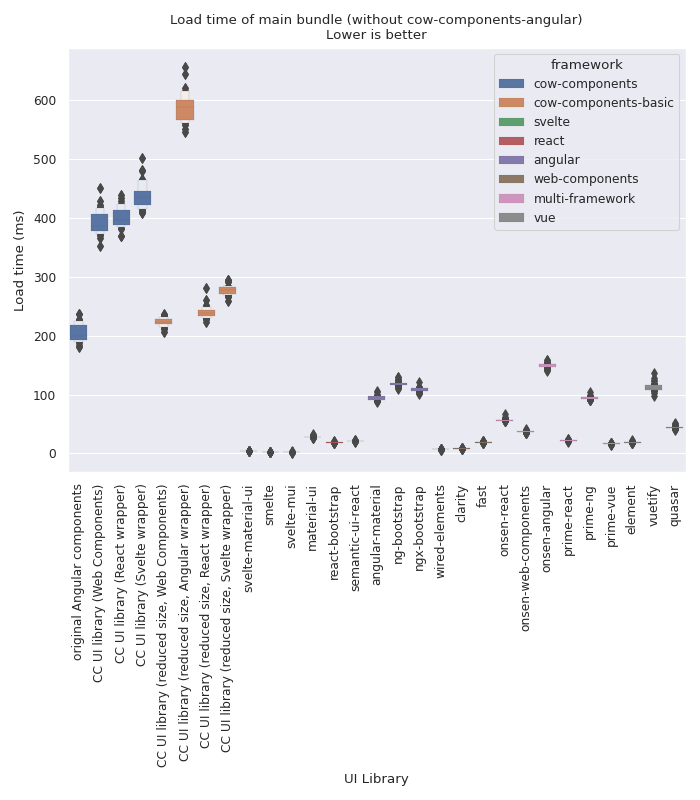
\includegraphics[width=\columnwidth]{plots/load-time-all-no-angular.png}
  \caption{Load time of the main JS bundle (without Angular wrapper).}
  \label{fig:results:load-time-all-no-angular}
  \centering
\end{figure}

\begin{figure}[h]
  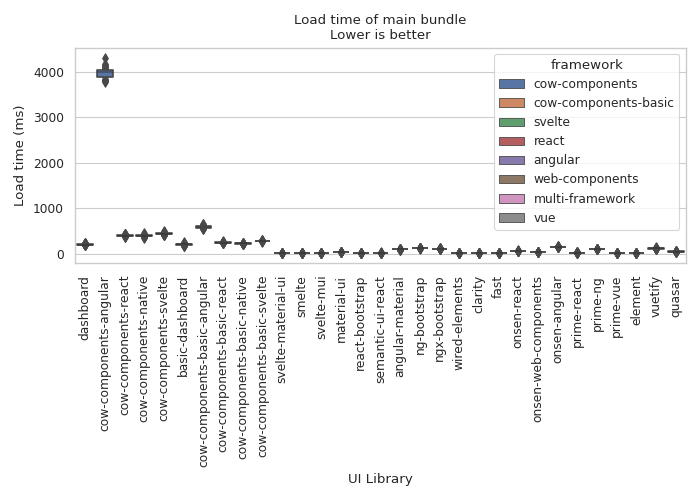
\includegraphics[width=\columnwidth]{plots/load-time-all.png}
  \caption{Load time of the main JS bundle.}
  \label{fig:results:load-time-all}
  \centering
\end{figure}

\section{Bundle Size}
Bundle size is a more abstract representation of the previous metric, allowing us to take a look at the impact of just the bundle size itself. This excludes any performance impact that can be attributed to poorly optimized code. This also allows us to look at what the performance impact of the Angular wrapper would be if there was no issue with the AOT compilation.

\begin{figure}[h]
  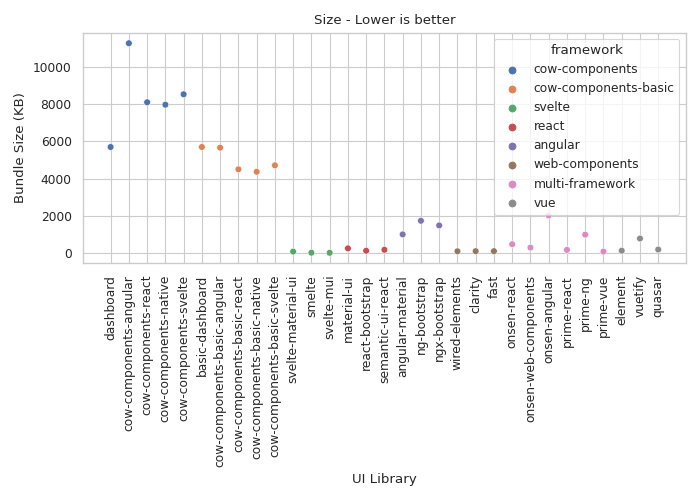
\includegraphics[width=\columnwidth]{plots/size.png}
  \caption{Size of the main JS bundle.}
  \label{fig:results:size}
  \centering
\end{figure}


The various bundle sizes can be found in Figure~\ref{fig:results:size}. We can first of all see that the bundle sizes correlate strongly with the load times. From this, we can conclude that they are an excellent representation of the load time metric. We find sizes average sizes of 57KB, 120KB, 204KB, and 385KB for Svelte, Web Component, React, and Vue UI libraries, respectively. As expected, Angular is by far the biggest, with a size of 1422KB. This same trend is also visible in our various wrappers. The Angular wrapper is by far the biggest, with a size of 11,251KB. With the strong correlation between load time and bundle size, we can conclude that a large part of the Angular wrapper's slow load time can be attributed to the large bundle size.

\section{Page Load Time}
The page load time metric should give us an idea of the real-world loading time of the CC UI library. As described in Chapter~\ref{chap:experimental-setup}, we replicated a page containing all components in the various distributions of the CC UI library. This means that all versions are rendering essentially the same page but in their own framework.

The resulting page load times can be found in Figure~\ref{fig:results:first-paint}. We have included both the \ver{First Paint} and \ver{First Contentful Paint} metrics, which are entirely the same for all the wrappers, only differing for the 30MHz dashboard. We find a first paint of 194ms and a first contentful paint of 233ms for the 30MHz dashboard. The Web Components version of the CC UI library has a first paint (and first contentful paint) of 25ms. This is 87\% faster than the 30MHz dashboard. This is likely because the dashboard also needs to run background tasks. These are tasks such as checking whether a user has logged in and fetching data. The CC UI library, on the other hand, has been stripped of this unneeded functionality. Apart from this, we can see a familiar trend of React and Svelte being slightly slower than the original, with first paint times of 618ms and 616ms, respectively. Finally, we find the Angular wrapper to have a first paint time of 2029ms.

\begin{figure}[h]
  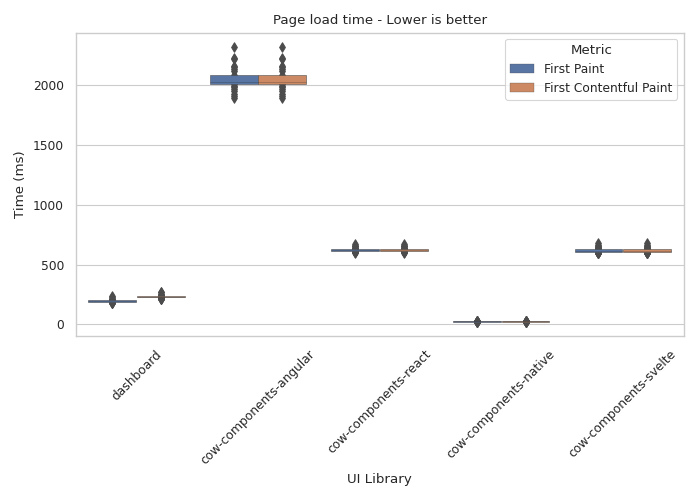
\includegraphics[width=\columnwidth]{plots/first-contentful-paint.png}
  \caption{First paint metrics for the various demo pages.}
  \label{fig:results:first-paint}
  \centering
\end{figure}

\section{Quality of Web Components}
In this section, we take a look at the quality of the Web Components in the CC UI library. Note that we essentially measure the quality of the original Angular components. This means that the conclusions drawn in this section only apply to the 30MHz codebase and will not be the same for other source codebases.

\begin{figure}[h]
  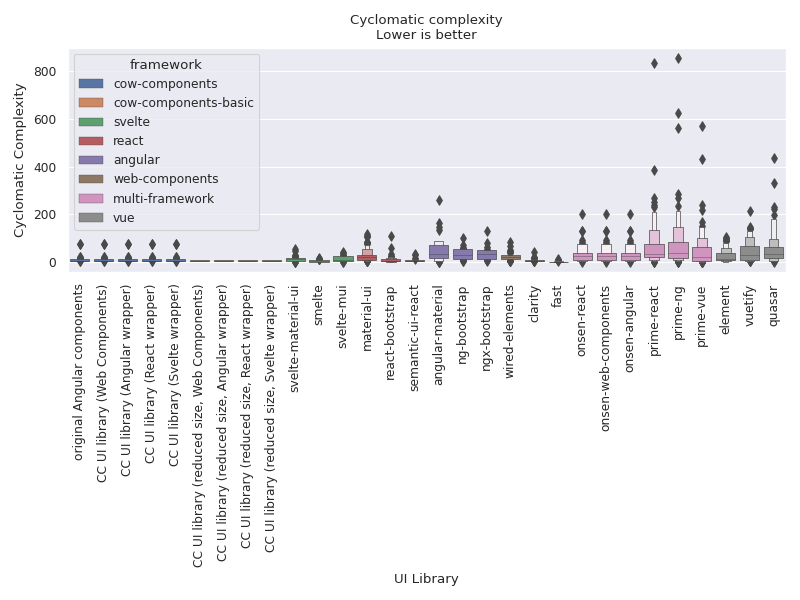
\includegraphics[width=\columnwidth]{plots/cyclomatic-complexity.png}
  \caption{Cyclomatic complexity of the various UI libraries.}
  \label{fig:results:cyclomatic-complexity}
  \centering
\end{figure}

\textbf{Cyclomatic complexity:} The cyclomatic complexities of the various UI libraries can be seen in Figure~\ref{fig:results:cyclomatic-complexity}. The cyclomatic complexity of the CC UI library is has a median value of 2 and a mean value of 10.4. The average cyclomatic complexity of the medians of all UI libraries is 17.5. Multi-framework UI libraries, in particular, have a very high cyclomatic complexity. The median cyclomatic complexity for all \ver{onsen}-based UI libraries is 22, while the cyclomatic complexities for \ver{prime-react}, \ver{prime-ng}, and \ver{prime-vue} are 31.5, 36, and 18 respectively. This makes sense since these libraries often try to share the source code between the various frameworks as much as possible, leading to many imports.

\begin{figure}[h]
  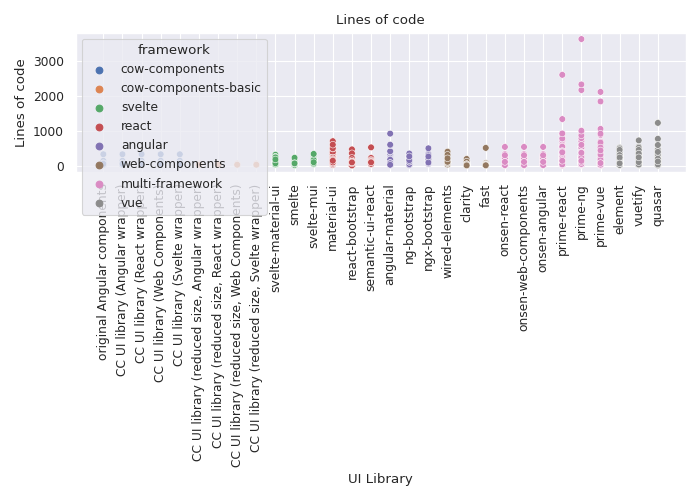
\includegraphics[width=\columnwidth]{plots/lines-of-code.png}
  \caption{Lines of code of the various UI libraries.}
  \label{fig:results:lines-of-code}
  \centering
\end{figure}

\textbf{Lines of code:} The amounts of lines of code can be seen in figure~\ref{fig:results:lines-of-code}. Again we see the same trend of the CC UI library being relatively low in complexity (and as such lines of code), with the median lines of code being 26. The average of the medians of all UI libraries is 108.75.

\begin{figure}[h]
  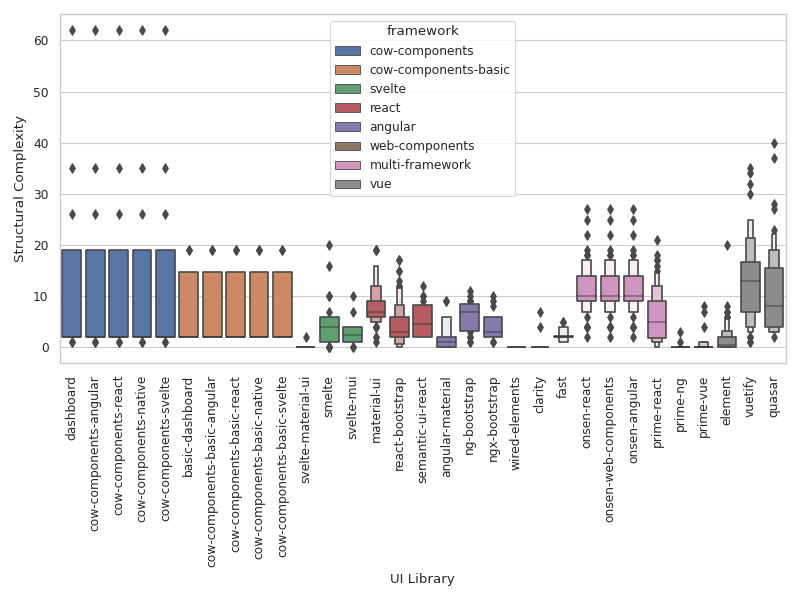
\includegraphics[width=\columnwidth]{plots/structural-complexity.png}
  \caption{Structural complexity of the various UI libraries.}
  \label{fig:results:structural-complexity}
  \centering
\end{figure}

\textbf{Structural complexity:} The structural complexities can be seen in figure~\ref{fig:results:structural-complexity}. This time there is a large variation in the structural complexity of CC UI library components, with the median being 2 and the average being 12.6. This outlier is likely to be the Chart component, which is by far the biggest component. The average of the other UI libraries' median structural complexity is 4.2. This suggests that the median structural complexity of the CC UI library is relatively low, which is good.

\begin{figure}[h]
  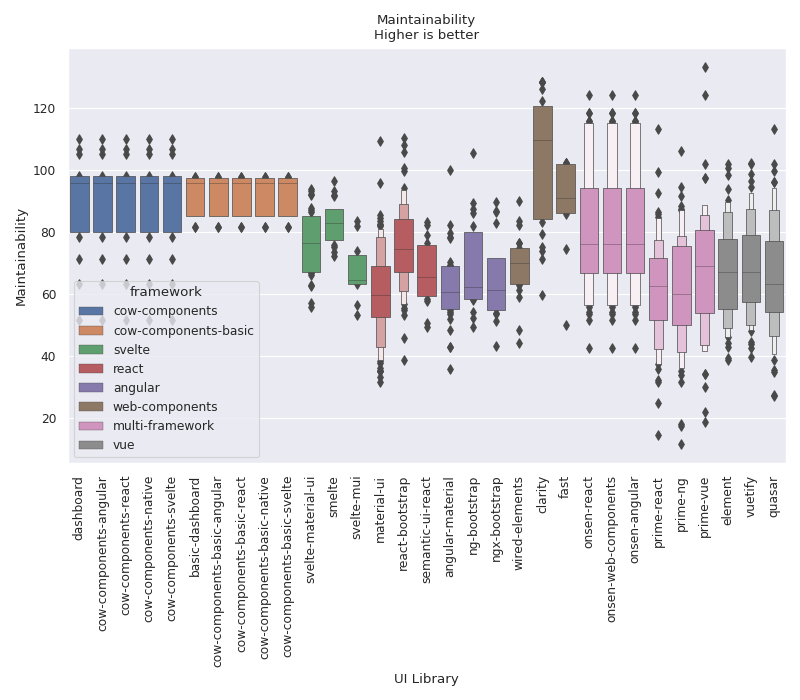
\includegraphics[width=\columnwidth]{plots/maintainability.png}
  \caption{Maintainability of the various UI libraries.}
  \label{fig:results:maintainabilty}
  \centering
\end{figure}

\textbf{Maintainability:} The maintainabilities can be seen in figure~\ref{fig:results:maintainabilty}. The median maintainability of the CC UI library is 96, with the average median maintainability of the UI libraries being 71. Higher maintainability is better, meaning the CC UI library scores quite well in this metric. All together, we can conclude that the quality of the CC UI library components (and as such, the Angular components they are based on) is quite high.

\section{Time spent on the project}\label{sec:results:time-spent}
While the technical results of this project are important, we also decided to take a look at the business side of this project. An important factor here would be the amount of effort required to complete this project. In total, this project took five months of fulltime-equivalent (FTE) to complete. An estimation would be that about one month was spent on Web Component related issues, three months on Angular related issues and one month on creating JS framework wrappers, and one month on other tasks such as creating a build pipeline and package distributions. Note that the time taken is entirely separate from the number of components in the resulting UI library, meaning an added component would not increase the time taken at all. Depending on the time required to build the UI library from scratch combined with the time taken to maintain the UI library and adding new components, this project could very well be worth it.